% Generated map data comes from ../proof-graph.yaml; source listings are live.
\providecommand{\srcroot}{../..}
\documentclass[10pt,a4paper]{article}
\usepackage[margin=1.8cm]{geometry}
\usepackage{fontspec}
\setmainfont{DejaVu Serif}
\setmonofont{DejaVu Sans Mono}[Scale=0.78]
\usepackage{amsmath,amssymb,booktabs,array,tabularx,fvextra,tikz,xcolor,xurl,hyperref}
\usetikzlibrary{arrows.meta,positioning}
\hypersetup{colorlinks=true,linkcolor=blue!50!black,urlcolor=blue!50!black,
 pdftitle={Symplectic Stafford: final paper and Lean correspondence},
 pdfauthor={Christopher Albert}}
\sloppy
\tikzset{
 >={Latex[length=2mm]},
 mapnode/.style={draw,rounded corners,align=center,text width=3.6cm,
   minimum height=0.85cm,font=\small},
 lean/.style={mapnode,fill=blue!12,very thick},
 lean-scaffold/.style={mapnode,fill=blue!5,densely dotted,very thick,font=\footnotesize},
 novel/.style={mapnode,fill=violet!8,double},
 gap/.style={mapnode,fill=orange!10,dashed,very thick},
 edge/.style={->,thick},
}
\newcommand{\backmap}{\hfill\hyperlink{proofmap}{[map]}}
\newcommand{\lean}[1]{\nolinkurl{#1}}
\newcolumntype{Y}{>{\raggedright\arraybackslash}X}
\title{Symplectic Stafford formalization\\[0.3em]
 \large Final-paper proof map and Challenge/Solution comparison}
\author{Christopher Albert}
\date{8 September 2026}
\begin{document}
% Generated by generate-proof-map.py; edit docs/proof-graph.yaml.
\begin{center}\hypertarget{proofmap}{}
{\Large Symplectic Stafford: proof map}\\[0.4em]
{\small LEAN: utility; LEAN-SCAFFOLD: conditional contract; NOVEL: paper candidate; GAP: open gate.}
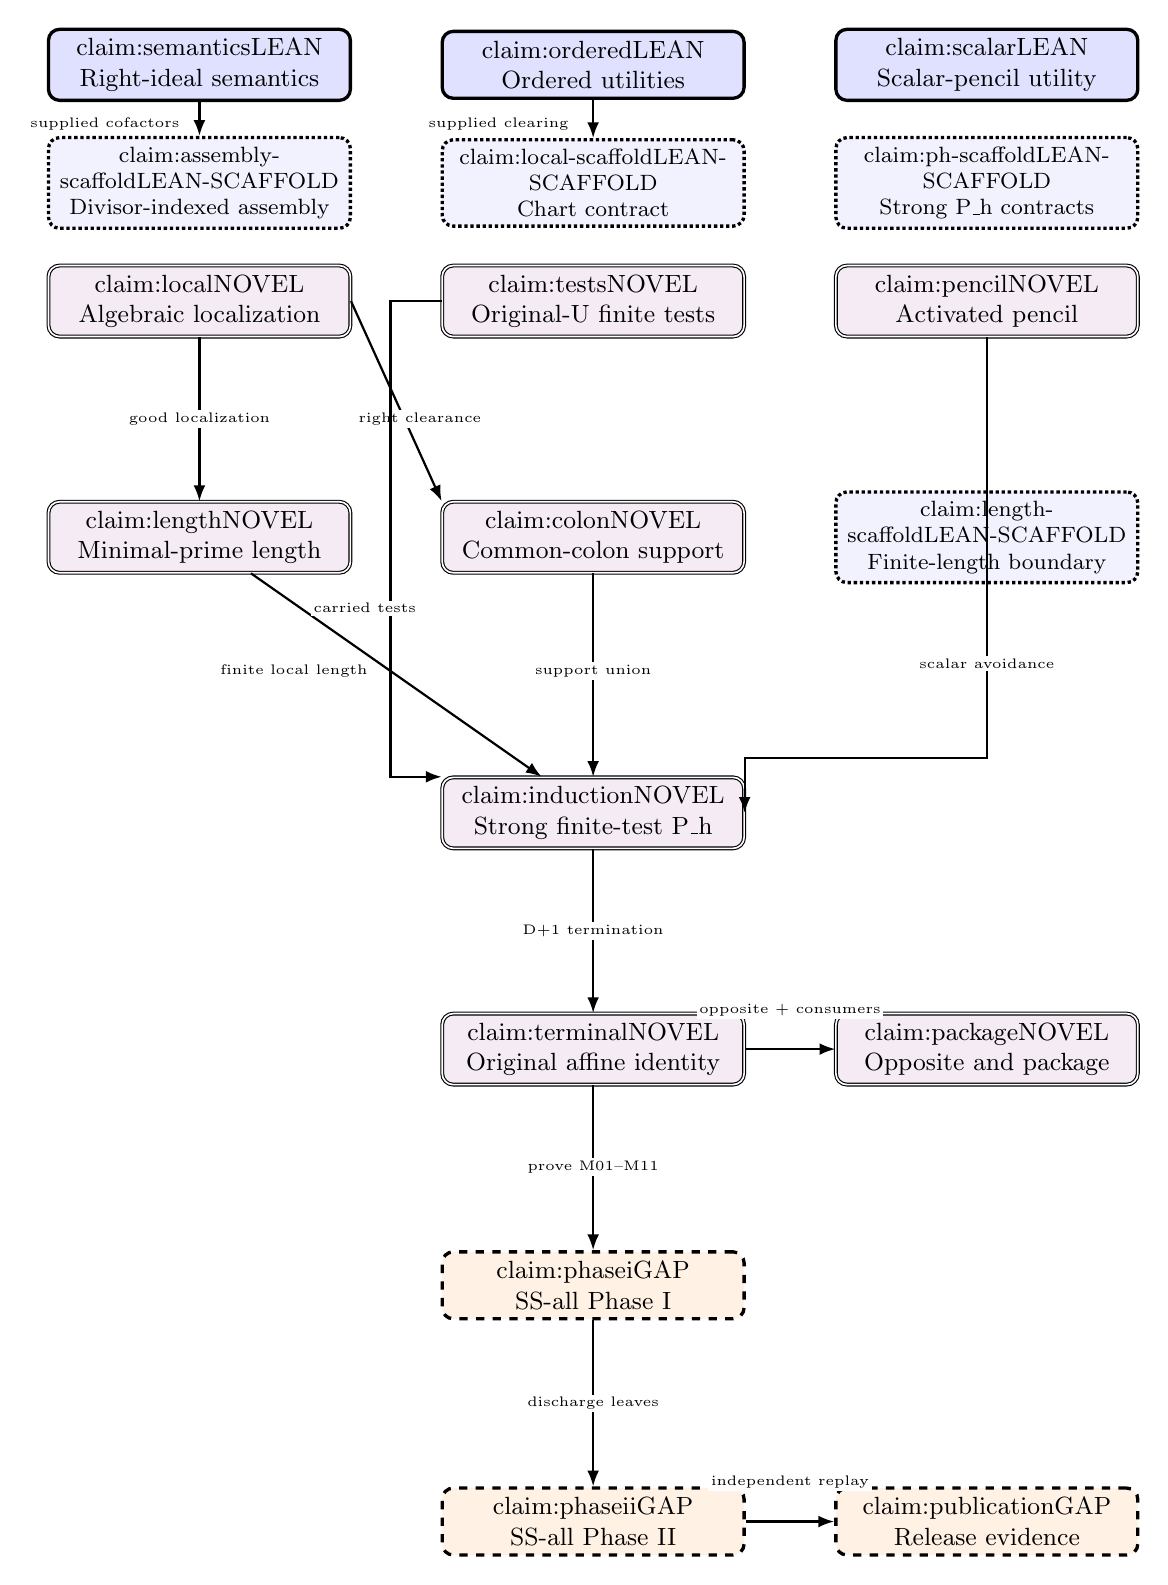
\begin{tikzpicture}[x=1cm,y=1cm]
\node[lean] (semantics) at (-5,20) {\hyperlink{claim:semantics}{LEAN\\Right-ideal semantics}};
\node[lean] (ordered) at (0,20) {\hyperlink{claim:ordered}{LEAN\\Ordered utilities}};
\node[lean] (scalar) at (5,20) {\hyperlink{claim:scalar}{LEAN\\Scalar-pencil utility}};
\node[lean-scaffold] (local-scaffold) at (0,18.5) {\hyperlink{claim:local-scaffold}{LEAN-SCAFFOLD\\Chart contract}};
\node[lean-scaffold] (assembly-scaffold) at (-5,18.5) {\hyperlink{claim:assembly-scaffold}{LEAN-SCAFFOLD\\Divisor-indexed assembly}};
\node[lean-scaffold] (ph-scaffold) at (5,18.5) {\hyperlink{claim:ph-scaffold}{LEAN-SCAFFOLD\\Strong P\_h contracts}};
\node[lean-scaffold] (length-scaffold) at (5,14) {\hyperlink{claim:length-scaffold}{LEAN-SCAFFOLD\\Finite-length boundary}};
\node[novel] (local) at (-5,17) {\hyperlink{claim:local}{NOVEL\\Algebraic localization}};
\node[novel] (tests) at (0,17) {\hyperlink{claim:tests}{NOVEL\\Original-U finite tests}};
\node[novel] (pencil) at (5,17) {\hyperlink{claim:pencil}{NOVEL\\Activated pencil}};
\node[novel] (length) at (-5,14) {\hyperlink{claim:length}{NOVEL\\Minimal-prime length}};
\node[novel] (colon) at (0,14) {\hyperlink{claim:colon}{NOVEL\\Common-colon support}};
\node[novel] (induction) at (0,10.5) {\hyperlink{claim:induction}{NOVEL\\Strong finite-test P\_h}};
\node[novel] (terminal) at (0,7.5) {\hyperlink{claim:terminal}{NOVEL\\Original affine identity}};
\node[novel] (package) at (5,7.5) {\hyperlink{claim:package}{NOVEL\\Opposite and package}};
\node[gap] (phasei) at (0,4.5) {\hyperlink{claim:phasei}{GAP\\SS-all Phase I}};
\node[gap] (phaseii) at (0,1.5) {\hyperlink{claim:phaseii}{GAP\\SS-all Phase II}};
\node[gap] (publication) at (5,1.5) {\hyperlink{claim:publication}{GAP\\Release evidence}};
\draw[edge] (semantics) -- (assembly-scaffold);
\node[fill=white,inner sep=1pt,font=\tiny] at (-6.2,19.25) {supplied cofactors};
\draw[edge] (ordered) -- (local-scaffold);
\node[fill=white,inner sep=1pt,font=\tiny] at (-1.2,19.25) {supplied clearing};
\draw[edge] (local) -- (length);
\node[fill=white,inner sep=1pt,font=\tiny] at (-5,15.5) {good localization};
\draw[edge] (local.east) -- (colon.north west);
\node[fill=white,inner sep=1pt,font=\tiny] at (-2.2,15.5) {right clearance};
\draw[edge] (length) -- (induction);
\node[fill=white,inner sep=1pt,font=\tiny] at (-3.8,12.3) {finite local length};
\draw[edge] (tests.west) -- ++(-0.65,0) |- (induction.north west);
\node[fill=white,inner sep=1pt,font=\tiny] at (-2.9,13.1) {carried tests};
\draw[edge] (pencil.south) |- ([yshift=0.7cm] induction.east) -- (induction.east);
\node[fill=white,inner sep=1pt,font=\tiny] at (5,12.4) {scalar avoidance};
\draw[edge] (colon) -- (induction);
\node[fill=white,inner sep=1pt,font=\tiny] at (0,12.3) {support union};
\draw[edge] (induction) -- (terminal);
\node[fill=white,inner sep=1pt,font=\tiny] at (0,9) {D+1 termination};
\draw[edge] (terminal) -- (package);
\node[fill=white,inner sep=1pt,font=\tiny] at (2.5,8.0) {opposite + consumers};
\draw[edge] (terminal) -- (phasei);
\node[fill=white,inner sep=1pt,font=\tiny] at (0,6) {prove M01–M11};
\draw[edge] (phasei) -- (phaseii);
\node[fill=white,inner sep=1pt,font=\tiny] at (0,3) {discharge leaves};
\draw[edge] (phaseii) -- (publication);
\node[fill=white,inner sep=1pt,font=\tiny] at (2.5,2) {independent replay};
\end{tikzpicture}\par\smallskip
{\scriptsize Graph SHA-256: \nolinkurl{2386286be0555daa6f2f34ca6d097a8021180dcea296fd188c00de98386476e0}}
\end{center}\clearpage

\maketitle

\begin{abstract}
The final paper gives a self-audited all-dimensional candidate for the
original-algebra identity \(1=dR+(B+Ha)dS\). This dossier records that proof's
dependencies, the partial Lean implementation, and the exact scope of the
current Challenge/Solution pair. The pair proves a definitional right-ideal
membership contract. A bounded independent paper-level audit found no invalid
bridge; formalization of the universal source producer and human review remain
open.
\end{abstract}

\section{Paper source and hypotheses}\label{sec:scope}\backmap

The mathematical source is the Markdown paper
\lean{docs/all-dimensional-symplectic-stafford-2026-09-08.md},
its parts I--III, and the two banked consequence documents in
\href{https://github.com/itpplasma/symplectic-stafford/tree/502b65a1dea53cac52220a08e321bfba525bc72e}
{the research repository at the frozen mathematical commit}.
The paper commit is
\lean{502b65a1dea53cac52220a08e321bfba525bc72e}; the terminal index,
roadmap and work ledger were refreshed at
\lean{e3c7077d3d51772d97d8e72bb219a8fc36765682}.
This TeX file is a comparison supplement, not a TeX transcription of a
manuscript. The map's structure follows the all-dimensional graph component,
with separate utility nodes for the actual Lean checkpoint.

Let \(k\) be an infinite characteristic-zero field and \(U\) a simple,
infinite-dimensional unital \(k\)-algebra with central scalar embedding.
Require an exhaustive separated nonnegative multiplicative filtration with
finite-dimensional pieces, \(U_0=k\), and commutative affine-domain
associated graded ring of finite Krull dimension \(D\). The final candidate
states that for every \(d\ne0\), arbitrary \(B\), and \(a\ne0\), there are
\(H,R,S\in U\) with
\[
  1=dR+\bigl((B+Ha)d\bigr)S.
\]
Setting \(B=0,a=1\) gives the same-divisor statement. Both occurrences of
\(d\) and every cofactor belong to the original \(U\). The symplectic class is
a subclass; no DL/Bn support lower bound or automatic tensor simplicity is
assumed by the core.

\section{The paper induction}\label{sec:architecture}\backmap

The predicate \(P_h\) quantifies over every divisor, every affine source
space \(B+Ua\), and every finite list of admissible local cyclic-generation
tests. It supplies a source passing those tests whose characteristic defect
dimension is at most \(D-h\), with the zero module assigned dimension \(-1\).

To prove \(P_{h+1}\), invoke only \(P_h\): first on \(d\), then on
\(d_1=dL_0\) after obtaining an actual relation \(FdL_0=dC_0\). The second
call carries the old minimal-module tests. The fixed right ideals are
\[
 K=\{s\in U:Gds\in dU\},\qquad J=dU+FdK.
\]
For an actual generator \(k\) and cofactor \(c\) satisfying \(Gdk=dc\), and
a central scalar \(t\), the ordered identity
\[
 Fdk=d(-tc)+(F+tG)dk
\]
places \(J\) in every member of the source pencil. Constant \emph{right}
denominator clearance yields
\(Z(U/J)\subseteq Z_d(F)\cup Z_{dL_0}(G)\).
Both lower-index bounds therefore control the common quotient. At its
minimal support primes the actual local modules have finite composition
length. The old/new split and one scalar avoiding all finitely many
exceptions remove every common minimal component while retaining the tests.
At \(P_{D+1}\), empty support gives zero quotient and literal original
cofactors \(R,S\). The recursion is on the index, not divisor degree.

Faithful algebraic Rees localization, local length, original-\(U\) finite
tests and the two-call successor remain project-owned proof obligations.
A theorem conditional on these constructions does not discharge them.

\section{Exact paper-to-Lean correspondence}\label{sec:comparison}\backmap

The formal statement vocabulary includes \lean{SameDivisorIdentity}; its
existence as a definition does not supply a producer. The semantic files
construct the right ideal
\[
 dU+(fd)U=\{x:\exists r,s,\ x=dr+(fd)s\},
\]
its relation-respecting quotient right-action operation and the opposite orientation. The current
Mathlib-only challenge isolates membership in this displayed carrier.
\lean{Semantics/RightIdealBridge.lean} supplies the ring-level wrapper only
after an explicit negation-closure proof and checks the quotient unit, zero,
multiplication, and action-respect laws; it does not turn arbitrary semiring
right ideals into ring ideals automatically.
\lean{Package/Opposite.lean} separately transports a supplied left certificate
to right S1 in the opposite ring (and conversely); a right certificate alone is
not silently treated as a left one.  \lean{Package/TerminalBoundary.lean}
records the exact terminal boundary: a supplied zero quotient or membership
witness yields literal original-\(U\) cofactors in the order
\(1=dR+(fd)S\), without constructing the support witness that the paper
needs.

The current \lean{AdmissibleSymplecticClass} is a historical,
dimension-parametric scaffold: it retains B2 fields and placeholder
proposition labels but does not yet encode the final all-dimensional
filtered-algebra class. The actual structural semantics remain an M01
obligation; the proved ring-level membership lemmas do not depend on this
scaffold.

\begin{center}
\begin{tabularx}{\textwidth}{@{}Y Y Y@{}}
\toprule
Paper requirement & Current Challenge & Current Solution\\
\midrule
Original carrier and order & Arbitrary Mathlib ring \(R\);
 \lean{generatedRightSet} & Identical definition;
 \(x=dr+(fd)s\)\\
Ordered membership & \lean{UniversalStatement} quantifies \(R,d,f,x\) &
 \lean{universalStatement} proves the equivalence by \lean{rfl}\\
Simple filtered-domain class & Absent from semantic challenge &
 No universal theorem supplied\\
Every nonzero divisor; affine source \(B+Ua\) & No source-existence
 quantifier & No \(H,R,S\) construction\\
Strong \(P_h\), localization and induction & Absent &
 Mandatory M02--M10 work remains\\
Opposite Stafford package & Absent & Orientation utility only;
 package requires its own endpoints\\
\bottomrule
\end{tabularx}
\end{center}

The identifier \lean{universalStatement} is universal over a
\emph{membership equivalence}, not the paper's source-existence theorem.
\lean{Challenge.lean} has one intentional statement placeholder.
\lean{Solution.lean} repeats its definitions without importing Challenge
and proves the membership statement. The configured Comparator can check
that pair's exact type and proof closure; it cannot establish correspondence
with the stronger paper target merely because both definitions have the
same name. A future terminal challenge must independently state the actual
class hypotheses and existential conclusion.

The ordered modules give affine identities and conditional finite
right-denominator clearance. The existing finite-pencil theorem treats
finitely many division-ring coordinates; general semisimple tops can have
repeated simple factors and matrix blocks. The new
\lean{FiniteLength/PencilBridge.lean} and
\lean{FiniteLength/ActivatedPencil.lean} record handed top-to-cyclic bridges
and finite forbidden-scalar avoidance, while
\lean{Source/OriginalTestContract.lean} records the exact original-\(U\) finite
test/source witness shape. \lean{Filtered/ReesBasic.lean} proves only raw
bounded-term coherence, \lean{Ordered/CommonColon.lean} keeps the K/J factor
order and central pencil identity explicit, and
\lean{Semantics/SupportDimension.lean} makes the bottom-support-to-quotient
boundary an input. \lean{Filtered/ReesAlgebra.lean} packages bounded
coefficient polynomials as a genuine subsemiring, while
\lean{Filtered/FiniteSupportDetection.lean} proves finite associated-top
extraction from supplied separatedness and exhaustion. All are conditional
consumers: arbitrary finite-length
activation, localization, support union and source-production proofs are still
required.

The remaining checked slices are listed explicitly in the claim register:
\lean{Semantics/RightIdealBridge.lean}, \lean{Filtered/ReesQuotient.lean},
\lean{Filtered/ReesAlgebra.lean}, \lean{Filtered/FiniteSupportDetection.lean},
\lean{Filtered/WeightedDetection.lean}, \lean{Source/DivisionLLD.lean},
\lean{Source/DifferentialOreDescent.lean},
\lean{FiniteLength/MinimalPrimeLength.lean},
\lean{FiniteLength/MatrixPencil.lean}, \lean{FiniteLength/RadicalLift.lean},
\lean{Ordered/SupportUnion.lean},
\lean{Ordered/FiniteGenerationBridge.lean},
\lean{Induction/TestRetention.lean},
\lean{Induction/ConcreteSuccessor.lean}, and
\lean{Package/TerminalBoundary.lean}.  Each is a conditional utility or
terminal boundary; none constructs the missing universal producer.

Three \textbf{LEAN-SCAFFOLD} nodes record additional conditional interfaces.
\lean{Filtered/Localization.lean} preserves degree bounds under supplied
filtration and map data, and combines power right-clearability already
supplied by the certificate. It constructs no full-symbol Ore localization,
Rees algebra or support theory. \lean{Source/Assembly.lean} now includes
\lean{DivisorIndexedAssembly}: each nonzero divisor may have its own source,
with original cofactors supplied in an \lean{AssemblyWitness}. Its
\lean{sameDivisor} consumer extracts those witnesses; it does not construct
the assembly data. Finite-candidate and uniform-source variants remain
separate optional toy contracts.

\lean{Source/DifferentialOreDescent.lean} records the differential chart
hypotheses and proves a finite powered-cover clearing consumer in the original
ring, preserving the factor order.  Its chart-to-global bridge, central
parameter-field S1, and all source-selection hypotheses are supplied inputs.
Likewise, \lean{Induction/ConcreteSuccessor.lean} makes the old/new test
families and carried-list obligations finite and explicit, but its two lower
\(P_h\) calls and output remain supplied data.

\lean{Induction/StrongPh.lean} records affine membership, finite test lists,
integer defect bounds, both lower-index calls and a supplied successor
output. The equation \(D-(D+1)=-1\) is proved. Its
\lean{Induction/FiniteIndex.lean} composes supplied \(P_1\) and successor rules
to \(P_{D+1}\). \lean{strongPh_succ} selects the output of a supplied successor rule, while
\lean{terminal_extraction} requires both terminal \lean{StrongPh} and a
\lean{zero_extraction} interface. Local-test specification propositions,
generation predicates and defect data are still abstract inputs. The
geometric semantics, successor producer and zero-support-to-cofactor bridge
remain to be proved. These checkpoints leave M02--M11 open and do not
advance the release gates.

\section{Phase instructions and evidence}\label{sec:phases}\backmap

\lean{docs/phase-instructions.md} gives the final-paper M01--M11 ledger.
Phase I discharges every project-owned step in the selected terminal
declaration's transitive closure. Individually audited literature leaves
alone may remain, each with its exact statement, source, wrapper and axiom
entry. Phase II replaces these leaves too, with transitive logical axioms
contained in \(\{\mathsf{propext},\mathsf{Classical.choice},\mathsf{Quot.sound}\}\).

The short-algebra, finite-module, filtered-localization, assembly and
package/model lanes may run concurrently on disjoint files. The controller
owns integration and phase promotion. Audit dependent definitions, instances,
wrapper hypotheses and imports; compare the exact terminal type independently.
Record the base commit and patch digest for uncommitted frozen review inputs.

Historical fourfold assembly, DL/Bn lower bounds and singularity catalogues
are optional for this terminal proof unless a named consumer uses them.
Concrete models still require their actual hypotheses, and physical Morita
applications require an actual algebraic progenerator. Arbitrary-projective
freeness and rank-one cancellation are outside the claimed package.

\section{Dependency and release record}\label{sec:release}\backmap

The dependency family uses Lean \lean{leanprover/lean4:v4.33.0} and
Mathlib's v4.33.0 revision
\lean{db584cd6d46c92f209a44c0f1c829460d327499d}.
The Stafford38 public main revision checked on 8 September 2026 is
\lean{e77e176c381ca2d6b20c030f9227f1b031415d2e}.
AlgebraicAnalysis public main is pinned at
\lean{46f2c819deca0e9735a436bed94ebed03ae35090}; this head was checked from
an isolated clone before the downstream replay.
The actual build pins are included below directly from the lock configuration;
dependency migration is complete only when manifest consistency and downstream
builds pass.

\VerbatimInput[fontsize=\scriptsize,breaklines=true,breakanywhere=true,
 frame=lines]{\srcroot/lakefile.toml}

The companion follows the Stafford38 and Global Stafford dossier pattern:
a claim map, explicit object/statement comparison, live Challenge/Solution
listings and replay evidence. It does not inherit either project's
verification status. In this workspace,
\lean{scripts/verify.sh --phase-i} checks the implemented checkpoint only.
Its name does not certify the terminal Phase-I gate.

Publication remains disabled in \lean{release-gates.yaml}. The release
runbook requires an immutable clean source commit, complete endpoint and
axiom evidence, independent semantic and kernel replay, and the separate
publication decision. The source and future release artifacts use the
repository's Apache-2.0 license; no DOI, public visibility change or Palomar
registration is claimed here.

\section{Claim register}\label{sec:claims}
\subsection{Right-ideal semantics}\hypertarget{claim:semantics}{}\backmap
\textbf{LEAN.} Literal ordered membership, quotient right action and opposite orientation in the original ring. The historical dimension-parametric B2/Prop-label class scaffold is not the final all-dimensional class; its structural M01 encoding remains open.

\emph{Source:} SymplecticStafford/Semantics/Contract.lean; SymplecticStafford/Semantics/S1Consequences.lean.
\emph{Review:} Implemented checkpoint; replay logs and precise types govern its scope.

No incoming claim dependency in this graph.
\subsection{Ordered utilities}\hypertarget{claim:ordered}{}\backmap
\textbf{LEAN.} Affine expansion and conditional finite constant-right-denominator clearing; no claim of an Ore structure or support theorem.

\emph{Source:} SymplecticStafford/Ordered/Affine.lean; SymplecticStafford/Ordered/RightClear.lean.
\emph{Review:} Implemented checkpoint; replay logs and precise types govern its scope.

No incoming claim dependency in this graph.
\subsection{Scalar-pencil utility}\hypertarget{claim:scalar}{}\backmap
\textbf{LEAN.} Finite exceptional scalars for finitely many division-ring coordinates; PencilBridge conditionally transfers this through a supplied top comparison/reflection. Constructing that comparison and the general activated finite-length bridge remains open.

\emph{Source:} SymplecticStafford/FiniteLength/Pencil.lean; SymplecticStafford/FiniteLength/PencilBridge.lean.
\emph{Review:} The coordinate theorem is implemented; CyclicTopBridge is a conditional consumer. Replay logs and precise types govern both scopes.

No incoming claim dependency in this graph.
\subsection{Chart contract}\hypertarget{claim:local-scaffold}{}\backmap
\textbf{LEAN-SCAFFOLD.} A supplied exhaustive multiplicative filtration and map preserve degree bounds; assuming chart-wide power right-clearability gives finite common right clearance. This constructs no full-symbol Ore set, Rees algebra, support theory or faithful localization.

\emph{Source:} SymplecticStafford/Filtered/Localization.lean.
\emph{Review:} Conditional checkpoint consumer; right\_clearable is an input field. M02–M05 remain open.

Dependencies: \hyperlink{claim:ordered}{Ordered utilities}.
\subsection{Divisor-indexed assembly}\hypertarget{claim:assembly-scaffold}{}\backmap
\textbf{LEAN-SCAFFOLD.} Given DivisorIndexedAssembly with a source and literal original cofactors for every nonzero divisor, extract SameDivisorS1. Sources may depend on d. OriginalTestContract records the M06 original-U finite-test/source witness shape and routes only a supplied composite producer to this consumer. This supplies no instance or producer; finite CandidateFamily and uniform SingleSourceAssembly are optional toy contracts.

\emph{Source:} SymplecticStafford/Source/Assembly.lean; SymplecticStafford/Source/OriginalTestContract.lean.
\emph{Review:} Conditional checkpoint consumer of supplied identity fields; M06 and M08–M11 remain open.

Dependencies: \hyperlink{claim:semantics}{Right-ideal semantics}.
\subsection{Strong P\_h contracts}\hypertarget{claim:ph-scaffold}{}\backmap
\textbf{LEAN-SCAFFOLD.} Record affine source membership, finite lists of abstract generation tests, integer defect bounds, both lower-index calls and supplied successor output. Prove D-(D+1)=-1 and conditionally extract original cofactors from a supplied terminal StrongPh and zero\_extraction interface.

\emph{Source:} SymplecticStafford/Induction/StrongPh.lean.
\emph{Review:} Conditional checkpoint: localization/module specifications, defect and generation predicates, successor output and zero\_extraction are supplied. M09–M11 are not proved.

No incoming claim dependency in this graph.
\subsection{Algebraic localization}\hypertarget{claim:local}{}\backmap
\textbf{NOVEL.} Full homogeneous-symbol Ore localization, algebraic Noetherian Rees ring, good subquotients and faithful detection including negative degrees.

\emph{Source:} paper part I.1–I.4 (M02–M04).
\emph{Review:} Self-audited paper candidate; independent mathematical and human review pending.

No incoming claim dependency in this graph.
\subsection{Original-U finite tests}\hypertarget{claim:tests}{}\backmap
\textbf{NOVEL.} One source in B+Ua satisfies every prescribed finite local cyclic-generation test with arbitrary offsets and nonzero right tails.

\emph{Source:} paper part II.1–II.4 (M06).
\emph{Review:} Self-audited paper candidate; independent mathematical and human review pending.

No incoming claim dependency in this graph.
\subsection{Activated pencil}\hypertarget{claim:pencil}{}\backmap
\textbf{NOVEL.} In a fixed finite-length cyclic module, vL=0 and e=vB+uL imply generic central-scalar cyclicity of v+lambda*u, over noncommuting endomorphism division rings.

\emph{Source:} paper part II.5 (M07).
\emph{Review:} Self-audited paper candidate; independent mathematical and human review pending.

No incoming claim dependency in this graph.
\subsection{Minimal-prime length}\hypertarget{claim:length}{}\backmap
\textbf{NOVEL.} Any finite good-filtered module has finite local composition length at a minimal homogeneous characteristic prime.

\emph{Source:} paper part I.5 (M05).
\emph{Review:} Self-audited paper candidate; independent mathematical and human review pending.

Dependencies: \hyperlink{claim:local}{Algebraic localization}.
\subsection{Common-colon support}\hypertarget{claim:colon}{}\backmap
\textbf{NOVEL.} For FdL0=dC0, K=\{s:Gds in dU\} and J=dU+FdK, polynomial pencil containment and constant right clearing yield Z(U/J) contained in Z\_d(F) union Z\_(dL0)(G).

\emph{Source:} paper main 1 (M08).
\emph{Review:} Self-audited paper candidate; independent mathematical and human review pending.

Dependencies: \hyperlink{claim:local}{Algebraic localization}.
\subsection{Strong finite-test P\_h}\hypertarget{claim:induction}{}\backmap
\textbf{NOVEL.} For every divisor, affine source space and finite test list, P\_h gives defect dimension at most D-h. The successor uses only P\_h twice, on d and dL0, removes all common minimal components and retains all carried tests.

\emph{Source:} paper main 2–4 (M09–M10).
\emph{Review:} Self-audited paper candidate; independent mathematical and human review pending.

Dependencies: \hyperlink{claim:length}{Minimal-prime length}, \hyperlink{claim:tests}{Original-U finite tests}, \hyperlink{claim:pencil}{Activated pencil}, \hyperlink{claim:colon}{Common-colon support}.
\subsection{Original affine identity}\hypertarget{claim:terminal}{}\backmap
\textbf{NOVEL.} P\_(D+1) gives empty support, hence actual original-algebra cofactors with 1=dR+(B+Ha)dS for every nonzero d and a and arbitrary B.

\emph{Source:} paper main 5 (M11).
\emph{Review:} Self-audited paper candidate; independent mathematical and human review pending.

Dependencies: \hyperlink{claim:induction}{Strong finite-test P\_h}.
\subsection{Opposite and package}\hypertarget{claim:package}{}\backmap
\textbf{NOVEL.} Automatic opposite hypotheses and the banked two-sided generation, rank, splitting and rank-at-least-two cancellation implications.

\emph{Source:} paper main 6; part III.1; same-divisor-consequences.md; rank-splitting-and-cancellation-2026-09-07.md (M11).
\emph{Review:} Self-audited paper candidate; independent mathematical and human review pending.

Dependencies: \hyperlink{claim:terminal}{Original affine identity}.
\subsection{SS-all Phase I}\hypertarget{claim:phasei}{}\backmap
\textbf{GAP.} All project-owned M01–M11 steps proved in the actual terminal type; only precise audited literature leaves may remain.

\emph{Source:} docs/phase-instructions.md.
\emph{Review:} Open gate; no completion evidence claimed.

Dependencies: \hyperlink{claim:terminal}{Original affine identity}.
\subsection{SS-all Phase II}\hypertarget{claim:phaseii}{}\backmap
\textbf{GAP.} All remaining literature leaves discharged; terminal axiom closure contained in propext, Classical.choice and Quot.sound.

\emph{Source:} docs/phase-instructions.md.
\emph{Review:} Open gate; no completion evidence claimed.

Dependencies: \hyperlink{claim:phasei}{SS-all Phase I}.
\subsection{Release evidence}\hypertarget{claim:publication}{}\backmap
\textbf{GAP.} Complete independent semantic/kernel replay and separately authorized publication at an immutable commit.

\emph{Source:} release-gates.yaml; docs/release-runbook.md.
\emph{Review:} Open gate; no completion evidence claimed.

Dependencies: \hyperlink{claim:phaseii}{SS-all Phase II}.

Paper statements follow the graph component at mathematical source commit
\nolinkurl{502b65a1dea53cac52220a08e321bfba525bc72e}.
The current instruction snapshot is
\nolinkurl{e3c7077d3d51772d97d8e72bb219a8fc36765682}.


\appendix
\clearpage
\section{Challenge source}\label{sec:challenge}\backmap
The listing is read directly from the current file at build time.
\VerbatimInput[fontsize=\scriptsize,breaklines=true,breakanywhere=true,
 frame=lines,numbers=left]{\srcroot/Challenge.lean}

\section{Solution and Comparator configuration}\label{sec:solution}\backmap
\VerbatimInput[fontsize=\scriptsize,breaklines=true,breakanywhere=true,
 frame=lines,numbers=left]{\srcroot/Solution.lean}
\VerbatimInput[fontsize=\scriptsize,breaklines=true,breakanywhere=true,
 frame=lines]{\srcroot/comparator.json}
\end{document}
